\documentclass[pdf,mia,noFooter,slideColor,colorBG]{prosper}
%\documentclass[mia,noFooter]{prosper}

\usepackage{amsmath, amssymb}
\usepackage{epsfig}
\usepackage[dvips]{color}

\newcommand{\emphase}[1]{{\textcolor{blue}{{#1}}}}
\newcommand{\publi}[1]{{\textcolor{blue}{{\sl \normalsize #1}}}}
\renewcommand{\paragraph}[1]{{\large \bf  #1}}

%====================================
%====================================
\begin{document}
%====================================
%====================================
\title{Title}
\subtitle{Subtitles}
\author{Smurf}
\email{smurf@inra.fr}
\institution{INRA}

%\maketitle

%====================================
\begin{slide}{}
  \psline[linewidth=50pt,linecolor=white](-2,1.4)(10.3,1.4)
  \rput[lb](2.5cm,0.4cm){\includegraphics[width=5cm]{Page1_top.eps}}
  \rput[lb](-0.3cm,-1.4cm){\includegraphics[width=10.5cm]{logoMIA19x2.eps}}
  \rput[lb](0.8cm,-4.8cm){Evaluation of the MIA Department -- October 2006}
  \rput[lb](-1.8cm,-5.2cm){\rotatebox[origin=c]{0}{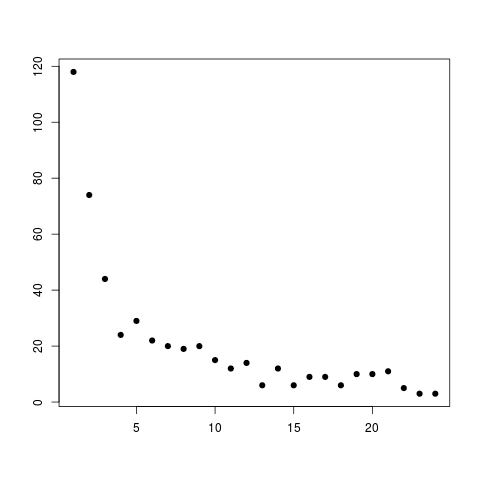
\includegraphics[width=2cm]{butterfly.eps}}}   
  \rput[lb](-2cm,-7.35cm){\includegraphics[width=13.7cm]{Page1_bottom.eps}}
 
  \rput[lb](0.5cm,-2.1cm){\Large\textbf{Statistics for Systems Biology}}
\end{slide}
%====================================

%====================================
\begin{slide}{SSB group}
\begin{itemize}
\item 3 MIA units: Jouy, Paris, Evry
\item 30 scientists
\item Regular meetings
\end{itemize}
\end{slide}
%====================================

%====================================
\begin{slide}{3 Major Research fields}
\vspace{0.5cm}
\begin{description}
\item[\paragraph{Sequence analysis:}] ~\\
  \emphase{Motifs} (discrete
  math., large deviation, Poisson approximation, scan statistics) \\
  \emphase{Local and alignment scores} (CUSUM processes, random walks,
  paired
  HMM) \\
  \emphase{Gene, motif and 2D structure prediction} (HMM, semi-Markov
  hidden models)
\end{description}
\end{slide}
%====================================

%====================================
\begin{slide}{}%3 Major Research Fields (2)}
\vspace{-0.75cm}
\begin{description}
\item[\paragraph{Microarray data:}] ~\\
  \emphase{Experimental design} (linear model) \\ 
  \emphase{Differential analysis} (multiple testing, mixture model) \\
  \emphase{Diagnostic} (supervised classification, dimension reduction, model
  selection) \\ 
  \emphase{Comparative Genomic Hybridisation} (breakpoints
  detection, mixed model)\\
  ~\\
\item[\paragraph{Biological networks:}] ~\\
  \emphase{Random graph models}
  (mixture models, variational methods, discrete math.), \\
  \emphase{Motifs} (Combinatorics, Poisson approximation), 
  \emphase{Network inference} (Graphical models, multiple testing)
\end{description}
\end{slide}
%====================================

%====================================
\begin{slide}{Two illustrations}
\begin{itemize}
\item Biological sequence analysis via HMM
  
% \begin{small}
%   \begin{equation*}
%     \frac{1}{\pi}=\sum_{n=0}^\infty \frac{(\frac{1}{4})_n(\frac{2}{4})_n(\frac{3}{4})_n}{n!^3}\bigl(2\sqrt{2}(1103+26390n)\bigr)\frac{1}{(99^2)^{2n+1}}
%   \end{equation*}
%   \end{small}
\item Statistical analysis of biological networks
\end{itemize}
\end{slide}
%====================================

%====================================
\begin{slide}{Sequence Analysis via HMM}
\end{slide}
%====================================

%====================================
\begin{slide}{\hspace{-6cm}Network Statistics }
  \vspace{-1cm}
  \begin{tabular}{cc}
    \hspace{-1cm}
    \begin{tabular}{p{3cm}}
      \\ \\ \\ \\ \\ \\ \\
      Yeast protein interaction network. \\
      {\small \sl Barabasi, Nat. Genet., 04} \\ \\ \\
    \end{tabular}
    &
    \begin{tabular}{c}
      \epsfig{file = ../Figures/Barabasi6.ps, clip=, bbllx=39, bblly=466,
        bburx=351, bbury=754, width=8cm}
    \end{tabular}
  \end{tabular}
\end{slide}
%====================================

%====================================
\begin{slide}{Complex Systems}
Molecular biologists more and more face data with a network
structure:
\begin{enumerate}
\item protein interaction networks
\item gene regulation networks
\item metabolic networks
\end{enumerate}

Statistical tools are needed
\begin{description}
\item[$(i)$] to understand and to lay out the global topology
of the graph \\
\item[$(ii)$] and to detect unexpected local structures.
\end{description}
\end{slide}
%====================================

%====================================
\begin{slide}{Our Contributions}
\begin{description}
\item[$(i)$] \paragraph{Models for random graphs} \\
  Random graphs are natural to describe such networks. \\
  Lack of models fitting the observed networks well. \\
  ~\\
\item[$(ii)$] \paragraph{Significant structures in a biological
    network} \\
  The search for unexpected patterns or characteristics (i.e.
  diameter) is the standard way to point out key features.
\end{description}
This field involves about \emphase{10 people} from Evry, Jouy and
Paris.
\end{slide}
%====================================

%====================================
\begin{slide}{A New Random Graph Model}
  \paragraph{Erd\"os Model.} All pairs of vertices have the \emphase{same
    probability} to be connected; All edges are independent. \\
  ~\\
  $\rightarrow$ Poor fit, probably due to some heterogeneity between
  the vertices (i.e. proteins, reactions, genes). \\
  ~\\
  \paragraph{Mixture Model.} Vertices are spread among \emphase{$Q$ groups}
  (with proportions $\alpha_q$); Vertices from groups $q$ and $\ell$
  are connected with probability $\pi_{q\ell}$. \\
  ~\\
  This includes the preferential attachment model: the groups
  correspond to the time when the vertices joined the network.
\end{slide}
%====================================

%====================================
\begin{slide}{Mixture Topologies}
%\vspace{-1cm}
\begin{tabular}{cc}
  \hspace{-1cm} 
  \begin{tabular}{c}
    Clusters (affiliation) \\
    \epsfig{file = ../figures/FigNetworks-Clusters-Col.eps,
      height=5cm, width=2.5cm, clip=, angle=270}    \\
    Stars (hubs) \\
    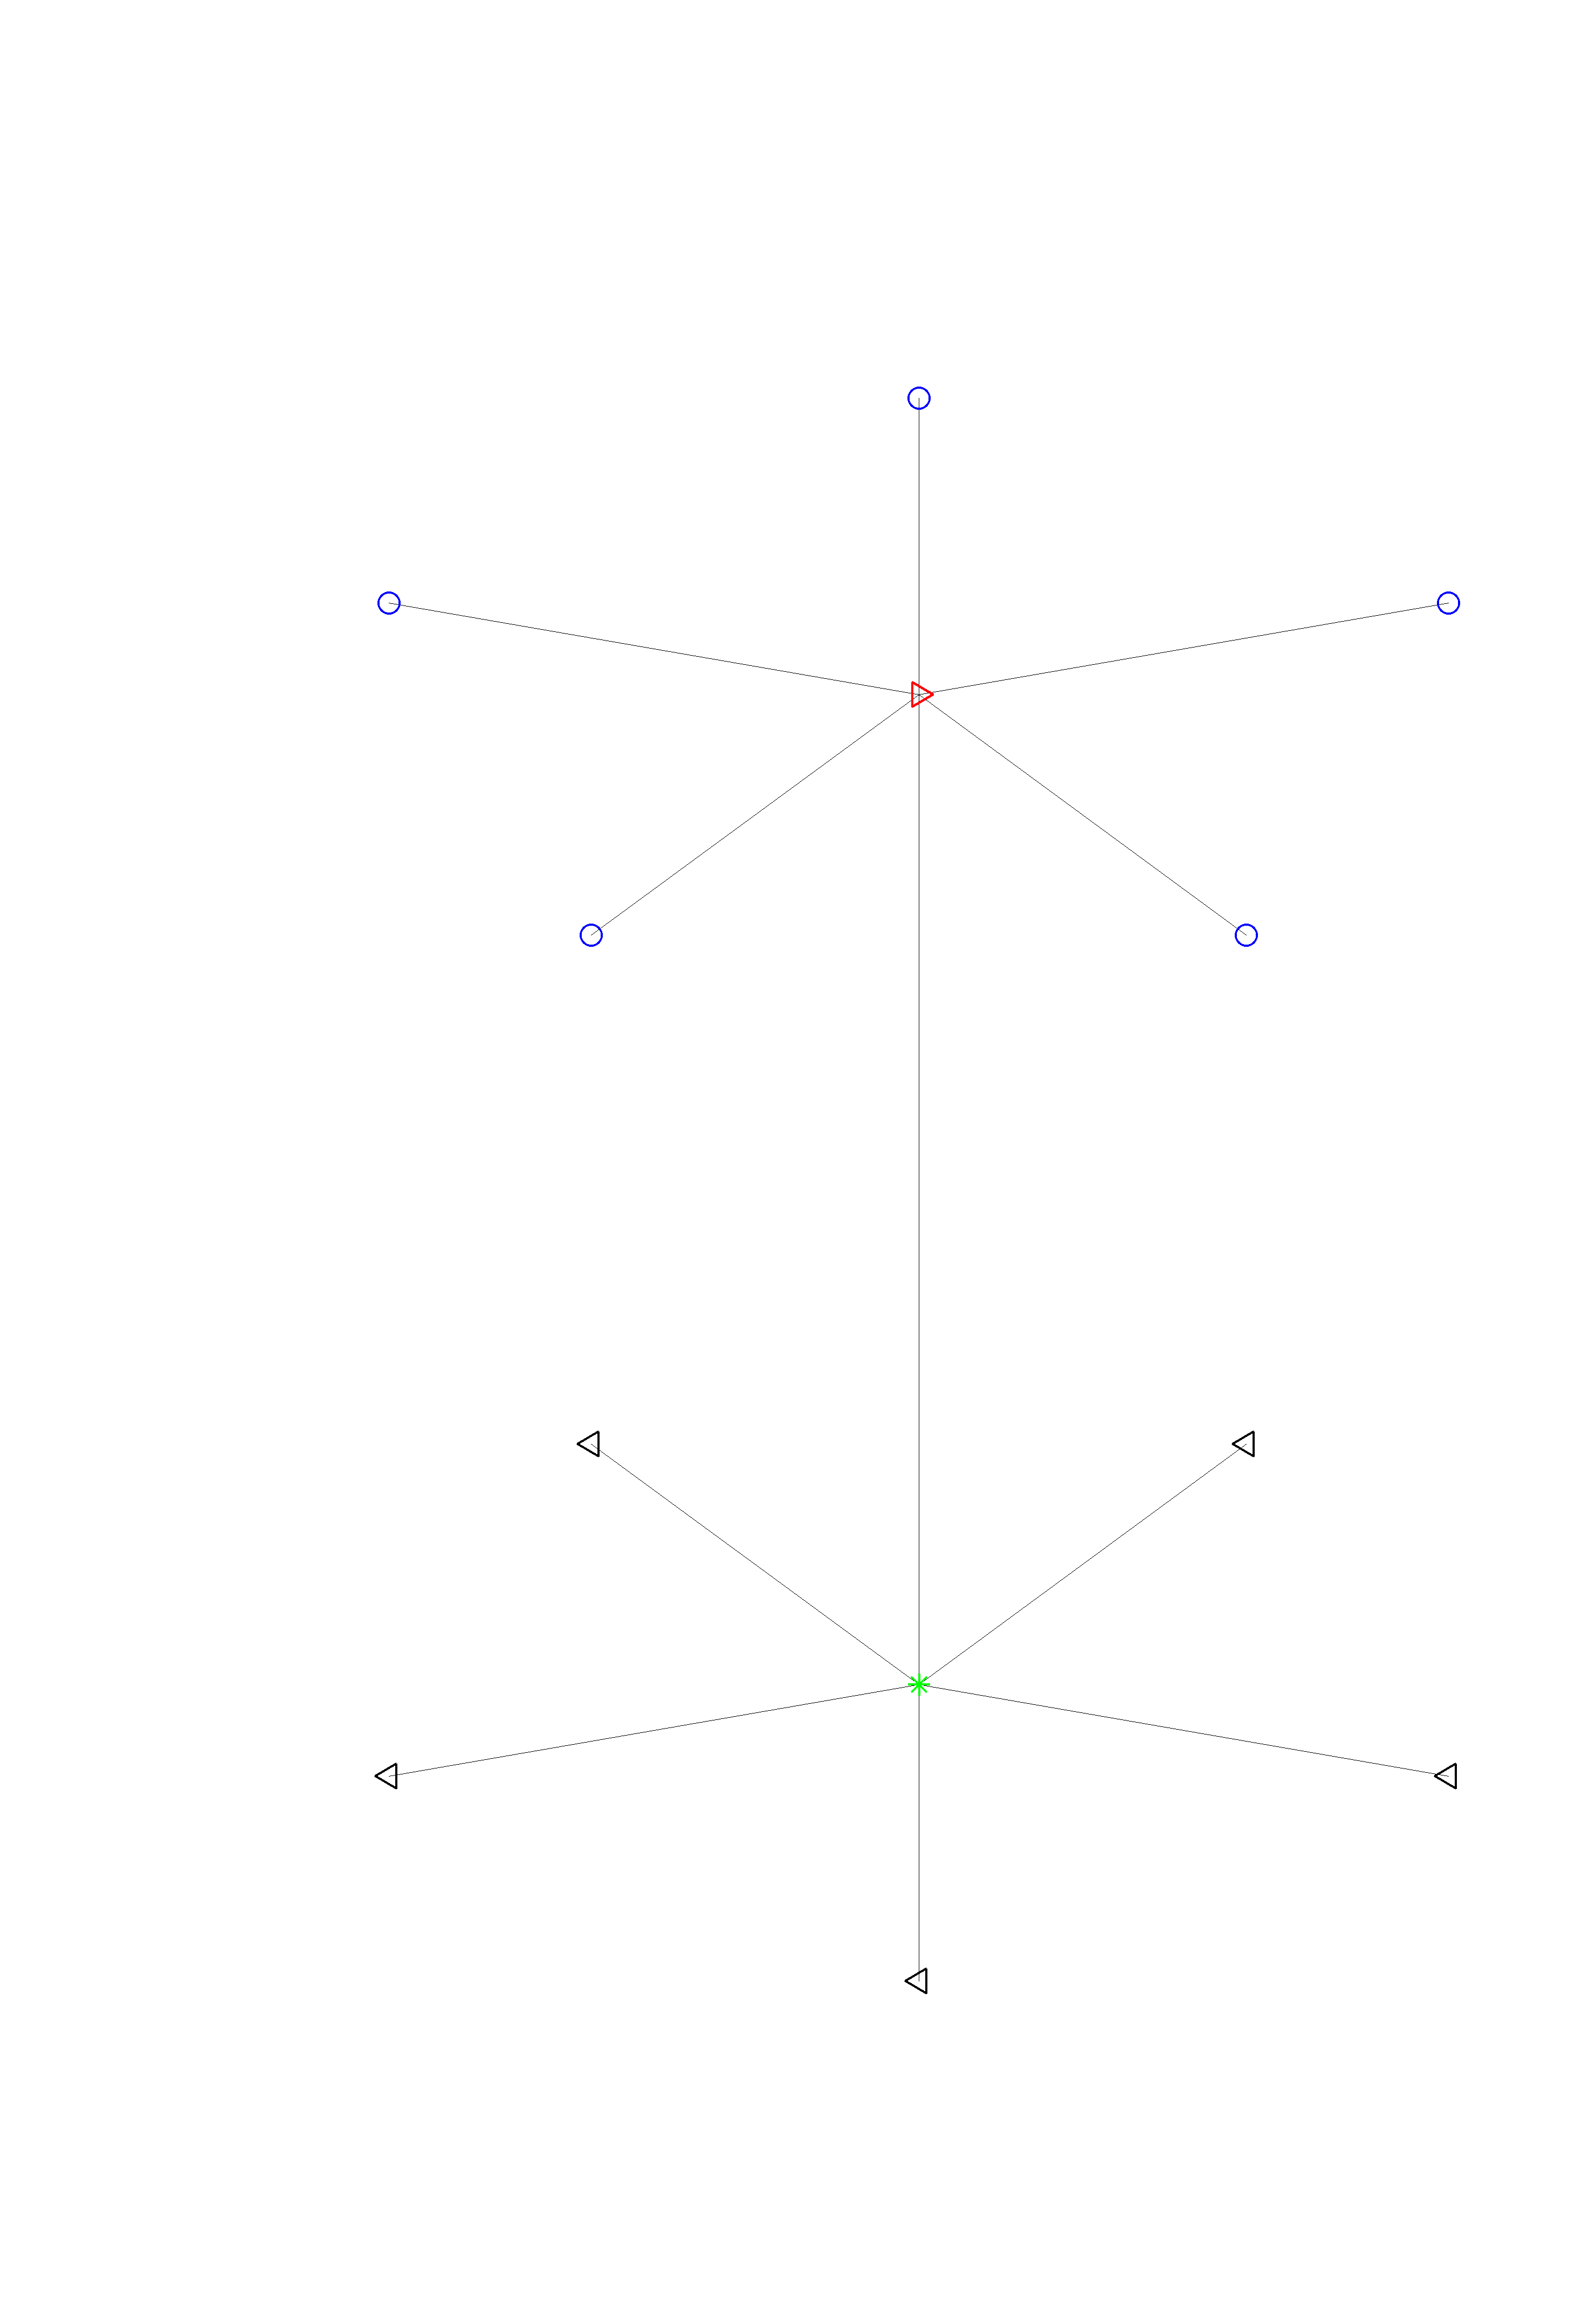
\epsfig{file = ../figures/FigNetworks-Star-Col.eps,
      height=5cm, width=2.5cm, clip=, angle=270}
    \end{tabular}
    &
    \begin{tabular}{c}
      Preferential \\ attachment \\
      \epsfig{file = ../figures/FigNetworks-PrefAtt-Col.eps, 
        height=5cm, width=5cm, clip=,}% angle=270}
    \end{tabular} 
  \end{tabular} 
\end{slide}
%====================================

%====================================
\begin{slide}{Parameter Estimation}
  \vspace{0.5cm}
  \paragraph{Standard strategy for mixture model: E-M.} \\
  The maximisation of the log-likelihood $\log P(X)$ of the observed
  edges $X$ involves the calculation of the conditional distribution
  of the unobserved vertex labels $Z$: $P(Z\;|\;X)$. \\
  ~\\
  \paragraph{E-M fails for random graphs.} \\
  All vertices are potentially connected so there is no local
  dependency: \\
  $\rightarrow$ The \emphase{neighbourhood of a vertex is the whole graph} \\
  $\rightarrow$ $P(Z\;|\;X)$ can  not be  computed \\
  $\rightarrow$ A new strategy is needed.
\end{slide}
%====================================

%====================================
\begin{slide}{Variational Approach}
  \paragraph{Lower bound for the likelihood.} \\
  We actually optimise
  $$
  \log P(X) - KL[P(Z\;|\;X), Q_R(Z)]
  $$
  where $Q_R$ is the \emphase{best approximation} of $P(Z\;|\;X)$
  within a class of 'nice' distributions:
  $$
  Q_R(Z) = \prod_i q(Z_i; \tau_i(X)).
  $$
  The multinomial parameters $\tau_i(X)$ can be interpreted as
  \emphase{posterior probabilities} for vertew $i$ to belong to each
  group.
\end{slide}
%====================================

%====================================
\begin{slide}{Estimation Algorithm}
  \begin{description}
  \item[\paragraph{Optimisation of $Q_R$.}] ~\\
    The optimal $\widehat{Q}_X$ is obtained with
    $\widehat{\tau}_i(X)$'s satisfying an explicit
    fix-point relation. \\
  \item[\paragraph{Parameter estimates.}] ~\\
    Given the $\widehat{\tau}_i(X)$, analytical expressions of
    $\widehat{\alpha}_q$ and $\widehat{\pi}_{q\ell}$ can be easily derived. \\
  \item[\paragraph{Model selection.}] ~\\
    A BIC-like criterion has been derived to choose the number of
    groups. \\ 
  \end{description}
  A \emphase{software} is available for both oriented and non-oriented
  graphs + \publi{under review at Stat. \& Comput. and PNAS}
\end{slide}
%====================================

%====================================
\begin{slide}{E. coli reaction network}
%\vspace{-1cm}
\hspace{-1.5cm}
\begin{tabular}{cc}
  \begin{tabular}{p{5cm}}
                                %\paragraph{Zoom (bottom left).} \\ 
                                %\\
    Submatrix of $\widehat{\pi}$:
    {\tiny      
      $$
      \begin{tabular}{c|cccc}
        $q, \ell$ & 1 & 7 & 10 & 16 \\
        \hline 
        1 & {\bf 1.0} \\ 
        7 & {\sl .11} & .65 \\ 
        10 & {\sl .43} & & .67  \\ 
        16 & {\bf 1.0} & {\sl .01} & & {\bf 1.0} \\
      \end{tabular}
      $$
      }
    Groups 1 and 16 both involve pyruvate; \\
    Only group 1 involves also
    CO2 (group 7) and acetylCoA (group 10).
                                %     \\ \\ 
  \end{tabular}
  &
  %\hspace{-1cm}
  \begin{tabular}{l}
    \epsfig{file = ../figures/Ecoli-Complet-ERMG-Ward-Q21_class.eps,
      height=5.5cm, width=5.5cm, clip=,bbllx=90, bblly=485, bburx=277,
      bbury=605.5} \\
    \publi{SSB + INRIA Helix: JOBIM 06}
  \end{tabular}  
%   \vspace{-2cm}
%   \\ \\ \\
%   \begin{tabular}{p{9cm}}
%     \paragraph{Vertices degree $K_i$.}  \\ \\ 
%     Mean degree in the last group:\\ 
%     $\overline{K}_{21} = 2.6$ \\ \\ \\
%   \end{tabular}
%   & 
%   \begin{tabular}{l}
%     \epsfig{file = ../figures/Ecoli-Complet-ERMG-Ward-Q21_class.eps,
%     width=8.5cm, height=3cm, clip=, bbllx=70, bblly=105, bburx=277,
%     bbury=245}   
%   \end{tabular}
\end{tabular}
\end{slide}
%====================================

%====================================
\begin{slide}{Network Motifs}
\begin{description}
\item[\paragraph{Regulatory motifs.}] ~\\
  $\begin{array}{ccc}
  \end{array}$
  Motifs may perform specific regulatory functions.
\item[\paragraph{Exceptional motifs.}] ~\\
  Motifs which occur more frequently than expected reflect functional
  or computational units which combine to regulate the cellular
  behaviour. \\
\item[\paragraph{Statistical significance.}] ~\\
  Need to evaluate 
  $
  \Pr\{N({\bf m}) \geq n_{obs}\}
  $
  where $N({\bf m}) = $ count of the motif ${\bf m}$ in a given
  network.
\end{description}
\end{slide}
%====================================

%====================================
\begin{slide}{State of the Art}
  \paragraph{Degree distribution fitting.} ~\\
  Consider a graph with random edges but where the degree of each
  vertex is fixed (and equal to the observed network). \\
  \begin{itemize}
  \item Shen-Orr \& al. (Nat. Genet. 01) estimate the distribution
    of $N({\bf m})$ using \emphase{simulations} \\
    $\longrightarrow$ heavy computational time.
  \item \publi{RevStat, 05} proposes \emphase{analytic formulas} for
    the moments \\
    $\longrightarrow$ difficult to implement because of the
    combinatorial complexity.
  \end{itemize}
\end{slide}
%====================================

%====================================
\begin{slide}{Stationary Models}
  \begin{tabular}{cc}
    \hspace{-1cm}
    \begin{tabular}{p{6cm}}
      Assume that the probability $\mu({\bf m})$ for motif ${\bf m}$ to occur
      \emphase{does not depend on the position} in the graph. \\
      \\
                                %\paragraph{Calculating the moments.}
      We can calculate the expected count \emphase{$\mathbb{E}
        N({\bf m})$} and variance of the count \emphase{$\mathbb{V}
        N({\bf m})$}. \\ \\ 
      $\mathbb{V} N({\bf m})$ depends on the expected count of
      {all possible overlaps} of the motif ${\bf m}$.\\ 
      (ex: ${\bf m} = {\Huge \times}$)
    \end{tabular}
    & 
    \hspace{-0.5cm}
    \begin{tabular}{c}
      \epsfig{file=
        /RECHERCHE/RESEAUX/Motifs/FIGURES/MotifStar4-Recouv3.eps,
        clip, width=4.6cm, height=6.5cm}
    \end{tabular}
  \end{tabular}
\end{slide}
%====================================

%====================================
\begin{slide}{Compound Poisson approx.}
  \paragraph{Approximate distribution of $N({\bf m})$.} ~\\
  The exact distribution of $N({\bf m})$ is still unknown. \\
  We look for an approximation involving only 2 parameters
  (corresponding to the 2 moments). \\
  ~\\
  \paragraph{Analogy with sequence motifs.} ~\\
  The compound (geometric) Poisson approximation outperforms other
  approximations for motif counts in sequences (e.g. DNA). \\ ~\\
  It assumes that the motif occurs in clumps, the number of clumps
  being Poisson and the clump size being Geometric.
  
\end{slide}
%====================================

%====================================
\begin{slide}{Examples}
  \begin{tabular}{cc}
    \hspace{-1cm}
    \begin{tabular}{p{5cm}}
      \paragraph{Geometric Poisson.}~\\
      Simulations show that it outperforms the Poisson and Gaussian
      approximations. \\ \\
      Although the geometric clump size is questionable for network
      motifs, the approximate $p$-values are accurate.
    \end{tabular}
    &
    \hspace{-0.5cm}
    \begin{tabular}{c}
      \epsfig{file=/RECHERCHE/RESEAUX/Motifs/FIGJJD-150506/fig11_200.eps, 
        bbllx=332, bblly=211, bburx=515, bbury=304, width=6cm,
        height=3.5cm, clip=} \\
      \textcolor{red}{\bf --} Gaussian, \textcolor{green}{\bf --}
        Compound Poisson \\
        \\
        \publi{submitted to Recomb 07}
    \end{tabular}
  \end{tabular}  
\end{slide}
%====================================

%====================================
\begin{slide}{Bipartite Graph}
  \begin{description}
  \item[\paragraph{Metabolic networks.}] Metabolic network involves 2
    different kinds of vertices: reactions and compounds. \\
  \item[\paragraph{Model.}] A stochastic model for such bipartite
    graph explains the properties of the projected graphs
    (\publi{submitted to Discr. Appl. Math.}).\\
  \item[\paragraph{Coloured motifs.}] Reaction motifs are connected
    sub-graphs involving reactions of a certain type (colour).
  \end{description }
\end{slide}
%====================================


%====================================
%====================================
\end{document}
%====================================
%====================================

